\documentclass[12pt, a4paper, oneside]{ctexart}
\usepackage{amsmath, amsthm, amssymb, bm, color, framed, graphicx, hyperref, mathrsfs}


% 超链接取消红框显示
\hypersetup{hidelinks} 

% 设置页边距
\usepackage{geometry}
\geometry{left=2.54cm,right=2.54cm,top=3.18cm,bottom=3.18cm}

\linespread{1.5}
\definecolor{shadecolor}{RGB}{241, 241, 255}


%-------------------------页眉页脚--------------
\usepackage{fancyhdr}
\usepackage{lastpage} % 获得总页数
\pagestyle{fancy}
\newcommand{\HRule}{\rule{\linewidth}{0.5mm}}%标题横线
\newcommand{\HRulegrossa}{\rule{\linewidth}{1.2mm}}


%-----------------------相关环境------------------
\newcounter{problemname}
\newenvironment{problem}{\begin{shaded}\stepcounter{problemname}\par\noindent\textbf{题目\arabic{problemname}. }}{\end{shaded}\par}

\newenvironment{solution}{\par\noindent\textbf{解答. }}{\par}

\newenvironment{note}{\par\noindent\textbf{题目\arabic{problemname}的注记. }}{\par}


%-----------------------伪代码------------------
\usepackage{algorithm}  
\usepackage{algorithmicx}  
\usepackage{algpseudocode}  
\floatname{algorithm}{Algorithm}  
\renewcommand{\algorithmicrequire}{\textbf{Input:}}  
\renewcommand{\algorithmicensure}{\textbf{Output:}} 
\usepackage{lipsum}  
\makeatletter
\newenvironment{breakablealgorithm}
{% \begin{breakablealgorithm}
		\begin{center}
			\refstepcounter{algorithm}% New algorithm
			\hrule height.8pt depth0pt \kern2pt% \@fs@pre for \@fs@ruled
			\renewcommand{\caption}[2][\relax]{% Make a new \caption
				{\raggedright\textbf{\ALG@name~\thealgorithm} ##2\par}%
				\ifx\relax##1\relax % #1 is \relax
				\addcontentsline{loa}{algorithm}{\protect\numberline{\thealgorithm}##2}%
				\else % #1 is not \relax
				\addcontentsline{loa}{algorithm}{\protect\numberline{\thealgorithm}##1}%
				\fi
				\kern2pt\hrule\kern2pt
			}
		}{% \end{breakablealgorithm}
		\kern2pt\hrule\relax% \@fs@post for \@fs@ruled
	\end{center}
}
\makeatother


%-----------------------代码环境------------------
\usepackage{listings}
\usepackage{xcolor}
\usepackage{ctex}
% 定义注释颜色
\definecolor{CommentGreen}{HTML}{00e500}

\lstset{
	basicstyle          =   \sffamily,          % 基本代码风格
	keywordstyle        =   \bfseries,          % 关键字风格
	commentstyle        =   \rmfamily\itshape,  % 注释的风格,斜体
	stringstyle         =   \ttfamily,  % 字符串风格
	flexiblecolumns,                % 别问为什么,加上这个
	numbers             =   left,   % 行号的位置在左边
	showspaces          =   false,  % 是否显示空格,显示了有点乱,所以不现实了
	numberstyle         =   \zihao{-5}\ttfamily,    % 行号的样式,小五号,tt等宽字体
	showstringspaces    =   false,
	captionpos          =   t,      % 这段代码的名字所呈现的位置,t指的是top上面
	frame               =   lrtb,   % 显示边框
}

\lstdefinestyle{Python}{
	language        =   Python, % 语言选Python
	basicstyle      =   \zihao{-5}\ttfamily,
	numberstyle     =   \zihao{-5}\ttfamily,
	keywordstyle    =   \color{blue},
	keywordstyle    =   [2] \color{teal},
	stringstyle     =   \color{magenta},
	commentstyle    =   \color{CommentGreen}\ttfamily,
	breaklines      =   true,   % 自动换行,建议不要写太长的行
	columns         =   fixed,  % 如果不加这一句,字间距就不固定,很丑,必须加
	basewidth       =   0.5em,
}

\renewcommand{\lstlistingname}{代码}


%-----------------------基本信息------------------
\title{\textbf{密码学课程作业} \textbf{\textrm{Hw-01}}} % 每次需要修改
\author{武桐西\quad 2112515\\
	信息安全一班
}
\date{\today}



% 正文部分
\begin{document}
	
	\maketitle
	 
	%-----------------------Header------------------
	\thispagestyle{fancy}
	\fancyhead{}
	\lhead{
\includegraphics[scale=0.1]{fig/Nankai_Logo.pdf} \kaishu{密码学} \textrm{Hw-01}} % 每次需要修改
	% \chead{}
	\rhead{\kaishu{武桐西} \textrm{2112515}}%加粗\bfseries 
	\lfoot{}
	\cfoot{\thepage\, / \pageref{LastPage}}
	\rfoot{}
	\renewcommand{\headrulewidth}{0.1pt}  
	\renewcommand{\footrulewidth}{0pt}%去掉横线
	\setlength{\textfloatsep}{10mm}%设置图片的前后间距
	
	% Begin Here:
	
	% 1.18
	\begin{problem}
		考虑下列定义在$ \mathbb{Z}_{2} $上的四级线性递归序列
		\[
		z_{i+4}=\left(z_{i}+z_{i+1}+z_{i+2}+z_{i+3}\right) \bmod 2
		\]
		$ i \geqslant 0 $。对其$ 16 $种可能的初始向量$ \left(z_{0}, z_{1}, z_{2}, z_{3}\right) \in \left( \mathbb{Z}_{2} \right)^{4} $,分别求出其生成的密钥流的周期。
	\end{problem}
	
	\begin{solution}
		作出该\textrm{FSR}的状态转移表,如表\ref{tab:FSR}所示。
		\begin{table}[H]
			\caption{状态转移表}
			\label{tab:FSR} \centering
			\begin{tabular}{|c|c||c|c|}
				\hline
				Current State & Next State & Current State & Next State \\
				\hline
				$ \left ( x_3, x_2, x_1, x_0 \right ) $ & $ \left ( x_3, x_2, x_1, x_0 \right ) $ & $ \left ( x_3, x_2, x_1, x_0 \right ) $ & $ \left ( x_3, x_2, x_1, x_0 \right ) $ \\
				\hline
				$ 0000 $ & $ 0000 $ & $ 1000 $ & $ 1100 $ \\ \hline
				$ 0001 $ & $ 1000 $ & $ 1001 $ & $ 0100 $ \\ \hline
				$ 0010 $ & $ 1001 $ & $ 1010 $ & $ 0101 $ \\ \hline
				$ 0011 $ & $ 0001 $ & $ 1011 $ & $ 1101 $ \\ \hline
				$ 0100 $ & $ 1010 $ & $ 1100 $ & $ 0110 $ \\ \hline
				$ 0101 $ & $ 0010 $ & $ 1101 $ & $ 1110 $ \\ \hline
				$ 0110 $ & $ 0011 $ & $ 1110 $ & $ 1111 $ \\ \hline
				$ 0111 $ & $ 1011 $ & $ 1111 $ & $ 0111 $ \\ \hline
			\end{tabular}
		\end{table}
		
		根据状态转移表,作出状态转移图,如图\ref{fig:FSR}所示。
		
		\begin{figure}[H]
			\centering
			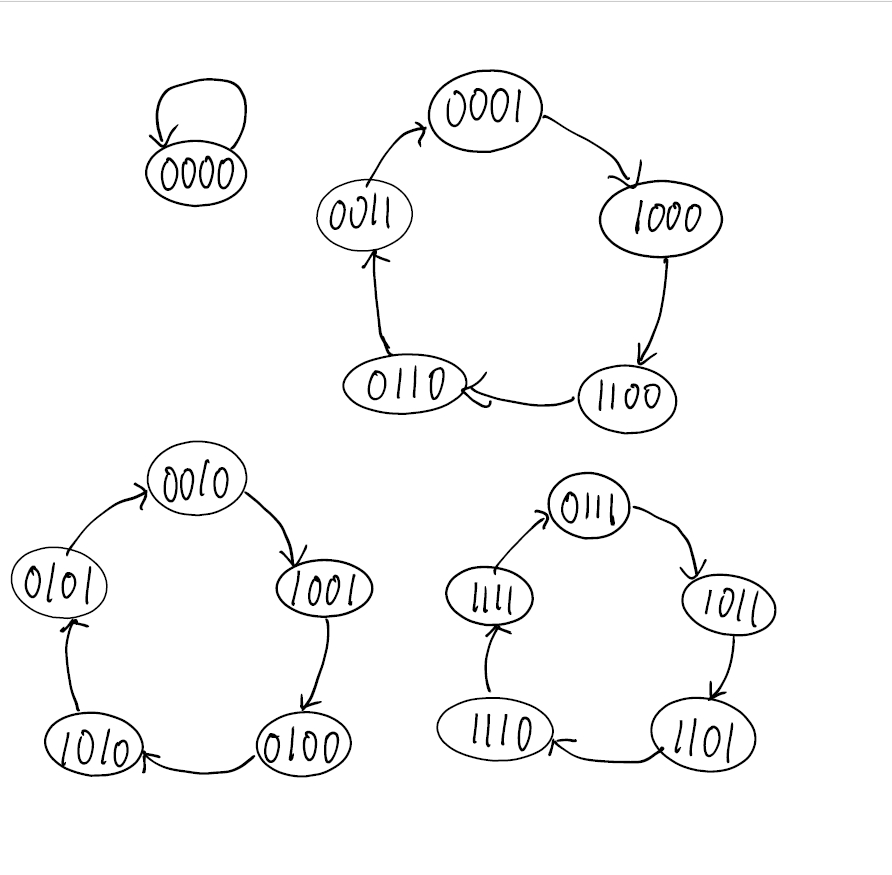
\includegraphics[width=0.7\linewidth]{fig/FSR}
			\caption{状态转移图}
			\label{fig:FSR}
		\end{figure}
		
		由图\ref{fig:FSR},当初始向量$ \mathbf{x} =  \left ( x_3, x_2, x_1, x_0 \right ) $为$ 0000 $时,其生成的密钥流的周期为$ 1 $,当初始向量$ \mathbf{x} =  \left ( x_3, x_2, x_1, x_0 \right ) $取其他$ 15 $个值时,其生成的密钥流的周期为$ 5 $.
		
	\end{solution}
	
	
	% 维吉尼亚密码
	\begin{problem}
		以下为维吉尼亚密码加密的密文,请破译其明文。
		
		K C C P K B G U F D P H Q T Y A V I N R R T M V G R K D N B V F D E T D G I L T X R G U D D K O T F M B P V G E G L T G C K Q R A C Q C W D N A W C R X I Z A K F T L E W R P T Y C Q K Y V X C H K F T P O N C Q Q R H J V A J U W E T M C M S P K Q D Y H J V D A H C T R L S V S K C G C Z Q Q D Z X G S F R L S W C W S J T B H A F S I A S P R J A H K J R J U M V G K M I T Z H F P D I S P Z L V L G W T F P L K K E B D P G C E B S H C T J R W X B A F S P E Z Q N R W X C V Y C G A O N W D D K A C K A W B B I K F T I O V K C G G H J V L N H I F F S Q E S V Y C L A C N V R W B B I R E P B B V F E X O S C D Y G Z W P F D T K F Q I Y C W H J V L N H I Q I B T K H J V N P I S T
		
	\end{problem}
	
	\begin{solution}
		
		$ (1) $首先采用\textbf{$ Kasiski $测试法}猜测该维吉尼亚密码使用的密钥的长度$ m $。
		
		首先搜索长度为$ 3 $的相同的密文段,并计算相同密文段之间的间距$ \delta_{i} $,得到对应的结果如下:
		
		密文段:['MVG', 'BVF', 'DDK', 'KFT', 'KFT', 'HJV', 'HJV', 'HCT', 'RLS', 'KCG', 'AFS', 'RWX', 'VYC', 'WBB', 'BBI', 'HJV', 'JVL', 'VLN', 'LNH', 'NHI', 'HJV'];
		其对应的间距:[156, 264, 198, 18, 156, 18, 138, 84, 18, 121, 60, 12, 42, 36, 36, 54, 54, 54, 54, 54, 12]。
		
		容易发现,密文段中出现次数最多的是\textrm{HJV},其在密文中共出现了$ 5 $次,其对应的间距分别为$ 18 $、$ 138 $、$ 54 $、$ 12 $,因此猜测密钥长度$ m $为它们的最大公因子$ \gcd{\left ( 18, 138, 54, 12 \right )} = 6 $,因此猜测密钥长度$ m = 6 $。
		
		上述分析过程的计算如代码\ref{code:guess_m.py}所示。
		
		\lstinputlisting[
		style=Python,
		caption={\textrm{guess\_m.py}: $ Kasiski $测试法猜测密钥长度$ m $},
		label=code:guess_m.py
		]{code/guess_m.py}
		
		
		为验证上述猜测的密钥长度的合理性,将密文分为$ m $组,计算每组的重合指数(Index of Coincidence)\footnote{该部分计算在代码\ref{code:index_of_coincidence_method.py}的前半部分。},结果表\ref{tab:Index_of_coincidence}所示。
		
		\begin{table}[H]
			\caption{密钥长度$ m = 6 $时,每组的重合指数}
			\label{tab:Index_of_coincidence} \centering
			\begin{tabular}{|c|c|c|c|c|c|c|}
				\hline
				分组 & 第$ 1 $组 & 第$ 2 $组 & 第$ 3 $组 & 第$ 4 $组 & 第$ 5 $组 & 第$ 6 $组 \\ \hline
				重合指数 & $ 0.063 $ & $ 0.084 $ & $ 0.049 $ & $ 0.065 $ & $ 0.043 $ & $ 0.073 $ \\ \hline
			\end{tabular}
		\end{table}
	
		可以看到每组的重合指数均比较接近$ 0.065 $,因此猜测密钥长度$ m = 6 $很可能是正确的。
		
		
		$ (2) $接下来采用重合指数法(Index of Coincidence Method)来猜测密钥$ K = \left ( k_{1}, k_{2}, k_{3}, k_{4}, k_{5}, k_{6} \right ) $。
		
		令$ p_{i} $表示第$ i $个英文字母出现的频率($ i = 0, 1, 2, \cdots , 25 $,即$ i \in \mathbb{Z}_{26} $),$ f_{i} $表示当前分组中第$ i $个英文字母出现的频数,$ n^{\prime} $表示当前分组的密文长度。
		假设$ 0 \leqslant g \leqslant 25 $,定义数值
		\begin{equation}
			\label{eq:M_g}
			M_{g}=\sum_{i=0}^{25} \frac{p_{i} f_{i+g}}{n^{\prime}}
		\end{equation}
		如果$ g=k_{i} $,则式(\ref{eq:M_g})退化为重合指数,应该有
		$ M_{g} \approx \sum_{i=0}^{25} p_{i}^{2} = 0.065 $。
		如果$ g \neq k_{i} $,则$ M_{g} $一般应该小于$ 0.065 $。\footnote{可由以下不等式得到:若$ a > b > 0 $,$ c > d > 0 $,则$ ac + bd > ad + bc $。}
		
		由上述分析可知,可以取每组中$ M_{g} $取最大值时对应的偏移$ g $作为该组的密钥$ k_{i} $,即$ k_{i} = \arg\max_{g} {M_{g}} $。
		
		
		综上,编程计算如代码\ref{code:index_of_coincidence_method.py}所示,得到解密后的明文如下:
		
		\begin{shaded}
			i l e a r n e d h o w t o c a l c u l a t e t h e a m o u n t o f p a p e r n e e d e d f o r a r o o m w h e n i w a s a t s c h o o l y o u m u l t i p l y t h e s q u a r e f o o t a g e o f t h e w a l l s b y t h e c u b i c c o n t e n t s o f t h e f l o o r a n d c e i l i n g c o m b i n e d a n d d o u b l e i t y o u t h e n a l l o w h a l f t h e t o t a l f o r o p e n i n g s s u c h a s w i n d o w s a n d d o o r s t h e n y o u a l l o w t h e o t h e r h a l f f o r m a t c h i n g t h e p a t t e r n t h e n y o u d o u b l e t h e w h o l e t h i n g a g a i n t o g i v e a m a r g i n o f e r r o r a n d t h e n y o u o r d e r t h e p a p e r
		\end{shaded}
		
		将该明文进行单词划分并添加标点符号,可以解析出如下信息:
		
		I learned how to calculate the amount of paper needed for a room when i was at school. You multiply the square footage of the walls by the cubic contents of the floor and ceiling combined, and double it. You then allow half the total for openings such as windows and doors. Then you allow the other half for matching the pattern. Then you double the whole thing again to give a margin of error, and then you order the paper.
		
		\lstinputlisting[
		style=Python,
		caption={\textrm{index\_of\_coincidence\_method.py}},
		label=code:index_of_coincidence_method.py
		]{code/index_of_coincidence_method.py}
		
		
	\end{solution}
	
\end{document}
